\RequirePackage{amsmath}
\documentclass{llncs}

\usepackage{amsmath}
\usepackage{amssymb}
\usepackage{array}
\usepackage{booktabs}
\usepackage{color}
\usepackage{float}
\usepackage{graphicx}
\usepackage{ifpdf}
\usepackage[utf8]{inputenc}
\usepackage{keyval}
\usepackage{listings}
\usepackage{moresize}
\usepackage{multirow}
\usepackage[numbers,sort&compress,square]{natbib}
\usepackage{paralist}
\usepackage{rotating}
\usepackage{soul}
% \usepackage[style=base]{subcaption}
\usepackage{srcltx}
\usepackage{url}
\usepackage[dvipsnames]{xcolor}
\usepackage{xspace}
\usepackage{wrapfig}
\usepackage{hyperref}
% \usepackage{caption}
\usepackage{enumitem}

\definecolor{listinggray}{gray}{0.95}
\definecolor{darkgray}{gray}{0.7}
\definecolor{commentgreen}{rgb}{0, 0.4, 0}
\definecolor{darkblue}{rgb}{0, 0, 0.6}
\definecolor{purple}{rgb}{0.6, 0, 0.6}
\definecolor{middleblue}{rgb}{0, 0, 0.75}
\definecolor{darkred}{rgb}{0.4, 0, 0}
\definecolor{brown}{rgb}{0.5, 0.5, 0}
\definecolor{dkgreen}{rgb}{0,0.5,0}
\definecolor{orange}{rgb}{1,.5,0}
\definecolor{dandelion}{cmyk}{0,0.29,0.84,0}

\lstset{ 
  backgroundcolor=\color{white},   % choose the background color; you must add \usepackage{color} or \usepackage{xcolor}; should come as last argument
  basicstyle=\ttfamily\footnotesize,        % the size of the fonts that are used for the code
  breakatwhitespace=false,         % sets if automatic breaks should only happen at whitespace
  breaklines=true,                 % sets automatic line breaking
  captionpos=b,                    % sets the caption-position to bottom
  commentstyle=\color{purple},    % comment style
  deletekeywords={...},            % if you want to delete keywords from the given language
  escapeinside={\%*}{*)},          % if you want to add LaTeX within your code
  extendedchars=true,              % lets you use non-ASCII characters; for 8-bits encodings only, does not work with UTF-8
  % frame=single,                    % adds a frame around the code
  keepspaces=true,                 % keeps spaces in text, useful for keeping indentation of code (possibly needs columns=flexible)
  keywordstyle=\color{orange},       % keyword style
  language=python,                 % the language of the code
  morekeywords={*,...},            % if you want to add more keywords to the set
  numbers=left,                    % where to put the line-numbers; possible values are (none, left, right)
  numbersep=5pt,                   % how far the line-numbers are from the code
  numberstyle=\tiny\color{darkgray}, % the style that is used for the line-numbers
  rulecolor=\color{black},         % if not set, the frame-color may be changed on line-breaks within not-black text (e.g. comments (green here))
  showspaces=false,                % show spaces everywhere adding particular underscores; it overrides 'showstringspaces'
  showstringspaces=false,          % underline spaces within strings only
  showtabs=false,                  % show tabs within strings adding particular underscores
  stepnumber=2,                    % the step between two line-numbers. If it's 1, each line will be numbered
  stringstyle=\color{commentgreen},     % string literal style
  tabsize=2,                       % sets default tabsize to 2 spaces
  % title=\lstname                   % show the filename of files included with \lstinputlisting; also try caption instead of title
}

\usepackage[normalem]{ulem}
\makeatletter
\def\cyanuwave{\bgroup \markoverwith{\lower3.5\p@\hbox{\sixly \textcolor{cyan}{\char58}}}\ULon}
\def\reduwave{\bgroup \markoverwith{\lower3.5\p@\hbox{\sixly \textcolor{red}{\char58}}}\ULon}
\def\blueuwave{\bgroup \markoverwith{\lower3.5\p@\hbox{\sixly \textcolor{blue}{\char58}}}\ULon}
\font\sixly=lasy6 % does not re-load if already loaded, so no memory problem.
\makeatother

\usepackage{pgfplots}
\pgfplotsset{compat=newest}
\usepgfplotslibrary{fillbetween}
\usetikzlibrary{patterns}

\usepackage{siunitx}
\DeclareSIUnit{\calorie}{cal}
\usepackage[outline]{contour}

\usepackage{makecell}

%\usepackage{xcolor}

\newif\ifdraft
\drafttrue
\ifdraft
 \newcommand{\N}[1]{\textbf{*** NOTE: #1}\xspace}
 \newcommand{\jhanote}[1]{ {\textcolor{red} { ***SJ: #1 }}}
 \newcommand{\mtnote}[1]{ {\textcolor{orange} { ***MT: #1 }}}
 \newcommand{\note}[1]{ {\textcolor{brown} { *** #1 }}}
 \newcommand{\jdnote}[1]{ {\textcolor{cyan} { ***JD: #1 }}}
 \newcommand{\dwwnote}[1]{ {\textcolor{blue} { ***DWW: #1 }}}
\else
 \newcommand{\N}[1]{}
 \newcommand{\jhanote}[1]{}
 \newcommand{\mtnote}[1]{}
 \newcommand{\jdnote}[1]{}
 \newcommand{\dwwnote}[1]{}
 \newcommand{\note}[1]{}
\fi

\newcommand{\cloud}{cloud\xspace}
\newcommand{\clouds}{clouds\xspace}
\newcommand{\pilot}{Pilot\xspace}
\newcommand{\pilots}{Pilots\xspace}
\newcommand{\pilotjob}{Pilot-Job\xspace}
\newcommand{\pilotjobs}{Pilot-Jobs\xspace}
\newcommand{\pilotcompute}{Pilot-Compute\xspace}
\newcommand{\pilotcomputedescription}{Pilot-Compute Description\xspace}
\newcommand{\pilotdescription}{Pilot-Description\xspace}
\newcommand{\pilotcomputes}{Pilot-Computes\xspace}
\newcommand{\pilotdata}{Pilot-Data\xspace}
\newcommand{\pilotdatadescription}{Pilot-Data Description\xspace}
\newcommand{\pilotdataservice}{Pilot-Data Service\xspace}
\newcommand{\pilotcomputeservice}{Pilot-Compute Service\xspace}
\newcommand{\computedataservice}{Compute-Data Service\xspace}
\newcommand{\computeunitdescription}{Compute-Unit Description\xspace}
\newcommand{\dataunitdescription}{Data-Unit Description\xspace}
\newcommand{\pilotmapreduce}{PilotMapReduce\xspace}
\newcommand{\mrmg}{MR-Manager\xspace}
\newcommand{\pstar}{P*\xspace}
\newcommand{\pd}{PD\xspace}
\newcommand{\pc}{PC\xspace}
\newcommand{\pcs}{PCs\xspace}
\newcommand{\pj}{PJ\xspace}
\newcommand{\pjs}{PJs\xspace}
\newcommand{\pds}{Pilot Data Service\xspace}
\newcommand{\computeunit}{Compute-Unit\xspace}
\newcommand{\computeunits}{Compute-Units\xspace}
\newcommand{\dataunit}{Data-Unit\xspace}
\newcommand{\dataunits}{Data-Units\xspace}
\newcommand{\du}{DU\xspace}
\newcommand{\dus}{DUs\xspace}
\newcommand{\dud}{DUD\xspace}
\newcommand{\cu}{CU\xspace}
\newcommand{\cus}{CUs\xspace}
\newcommand{\cud}{CUD\xspace}
\newcommand{\su}{SU\xspace}
\newcommand{\sus}{SUs\xspace}
\newcommand{\schedulableunit}{Schedulable Unit\xspace}
\newcommand{\schedulableunits}{Schedulable Units\xspace}
\newcommand{\cc}{c\&c\xspace}
\newcommand{\CC}{C\&C\xspace}
\newcommand{\up}{\vspace*{-1em}}
\newcommand{\upp}{\vspace*{-0.5em}}
\newcommand{\numrep}{8 }
\newcommand{\samplenum}{4 }
\newcommand{\tmax}{$T_{max}$ }
\newcommand{\tc}{$T_{C}$ }
\newcommand{\tcnsp}{$T_{C}$}
\newcommand{\bj}{BigJob\xspace}
\newcommand{\irods}{iRODS\xspace}

\newcommand{\I}[1]{\textit{#1}\xspace}
\newcommand{\B}[1]{\textbf{#1}\xspace}
\newcommand{\T}[1]{\texttt{#1}\xspace}
%\newcommand{\C}[1]{\textsc{#1}\xspace}

\newcommand{\mr}[1]{\multirow{2}{*}{#1}}%
\newcommand{\mc}[2]{\multicolumn{#1}{l}{#2}}

\lstdefinestyle{myListing}{
  frame=single,
  backgroundcolor=\color{listinggray},
  %float=t,
  language=C,
  basicstyle=\ttfamily \footnotesize,
  breakautoindent=true,
  breaklines=true
  tabsize=2,
  captionpos=b,
  aboveskip=0em,
  belowskip=-2em,
  %numbers=left,
  %numberstyle=\tiny
}

\lstdefinestyle{myPythonListing}{
  frame=single,
  backgroundcolor=\color{listinggray},
  %float=t,
  language=Python,
  basicstyle=\ttfamily \scriptsize,
  breakautoindent=true,
  breaklines=true
  tabsize=2,
  captionpos=b,
  %numbers=left,
  %numberstyle=\tiny
}



%  \setlength{\parskip}{0.05ex} % 1ex plus 0.5ex minus 0.2ex}
%  \setlength{\parsep}{0pt}
%  %\setlength{\headsep}{0pt}
%  \setlength{\topskip}{0pt}
%  \setlength{\topmargin}{0pt}
%  %\setlength{\topsep}{0pt}
%  \setlength{\partopsep}{0pt}

% This is now the recommended way for checking for PDFLaTeX:


\ifpdf
\DeclareGraphicsExtensions{.pdf, .jpg, .tif}
\else
\DeclareGraphicsExtensions{.ps,  .eps, .jpg}
\fi

\tolerance=1000
\hyphenpenalty=10




\title{Rapid, concurrent and adaptive extreme scale binding free energy calculation}

%\title{Concurrent Drug Binding Affinity Computations using Adaptive Simulations}

% \author{
%   \IEEEauthorblockN{Jumana Dakka, Vivek Balasubramanian, Matteo Turilli, Shantenu Jha}
%   \IEEEauthorblockA{RADICAL Laboratory, Electric and Computer Engineering,
%    Rutgers University, New Brunswick, NJ, USA}
% }

\begin{document}
\maketitle


%\author{Kristof Farkas-Pall, David W Wright, Shunzhou Wan, Peter V Coveney}
%\orcid{}
%\affiliation{%
%  \institution{UCL}
%  \streetaddress{20 Gordon Street}
%  \city{London}
  %\state{}
%  \country{UK}


%\renewcommand\shortauthors{Dakka, J. et al}

\begin{abstract}

The recently demonstrated ability to perform accurate, precise and rapid
computation of ligand binding strengths has driven interest in the use of
molecular simulations for applications in both computer-aided drug design and
patient specific medicine. Simulation protocols based on ensembles of multiple
runs of the same system provide an efficient method for producing robust free
energy estimate, and equally important statistical uncertainties. Variations
in the chemical and biophysical properties of different systems impact the
optimal protocol choice for different proteins and classes of drugs targetting
them. However, these are difficult to determine {\it a priori}, thus requiring
adaptive execution of a simulation workflows. We introduce the High-throughput
Binding Affinity Calculator (HTBAC) to enable the scalable, adaptive and
automated calculation of the binding free energy on high-performance computing
resources. We investigate weak scaling behaviour for screening sixteen drug
candidates concurrenlty using thousands of multi-stage pipelines on more than
32,000 cores. This permits a rapid time-to-solution that is essentially
invariant with respect to the calculation protocol, size of candidate ligands
and number of ensemble simulations. As such, HTBAC advances the state of the
scale and sophistication of binding affinity calculation. HTBAC uses readily
available building blocks to attain both workflow flexibility and performance;
our scaling experiments are performed on the Blue Waters machine at NCSA.

\end{abstract}


% To simply model building and simulation setup we developed an automation tool,
% the Binding Affinity Calculator (BAC). Building on this tool, to support the
% scalable, adaptive and automated calculation of the binding free energy on
% high-performance computing resources,


% \begin{abstract}
% Recent improvements in computational power and algorithm design mean that
% reliably quantifying ligand binding strength differences from molecular
% simulation is becoming a genuine possibility. These developments have led to
% increased interest in the use of molecular simulations for applications in both
% computer-aided drug design and patient specific medicine. We have previously
% demonstrated that simulation protocols based on ensembles of multiple runs of
% the same system provide an efficient method for producing robust free energy
% estimate, and equally important statistical uncertainties. Variations in the
% chemical and biophysical properties of different systems impact the optimal
% protocol choice for different proteins and classes of drugs targetting them.
% This leads to the necessity of automation and middleware solutions that allow
% adaptive execution of a wide range of simulation workflows. To support the
% scalable, adaptive and automated calculation of the binding free energy on
% high-performance computing resources, we introduce the High- throughput Binding
% Affinity Calculator (HTBAC). HTBAC uses a building block approach in order to
% attain both workflow flexibility and performance. We demonstrate close to
% perfect weak scaling to hundreds of concurrent multi-stage binding affinity
% calculation pipelines. This permits a rapid time-to-solution that is
% essentially invariant of the calculation protocol, size of candidate ligands
% and number of ensemble simulations. As such, HTBAC advances the state of the
% art of binding affinity calculations and protocols.
% \end{abstract}

% \keywords{binding free energy, binding affinity, drug binding, middleware}

%\maketitle

\section{Introduction}
Drug discovery and design is immensely expensive with one study putting the
current cost of each new therapeutic molecule that reaches the clinic at
US\$1.8 billion~\cite{Paul2010}. A diversity of computational approaches,
specifically binding free energy calculations which rely on physics-based
molecular dynamics simulations (MD) have been developed~\cite{Mobley2012} and
blind tests show that many have considerable predictive
potential~\cite{Mey2017,Yin2017}. The development of commercial approaches
that claim accuracy of below 1 kcal mol$^{-1}$~\cite{Wang2015} has led to
increased interest from the pharmaceutical industry~\cite{Ganesan2017} in
designing computational drug campaigns.

These improvements can be attributed to many advances in methodologies and
hardware. Specifically, ensemble-based binding free energy calculations,
which favor many shorter simulation trajectories over few longer simulations
have been shown to increase sampling efficiency whilst also reducing time to
insight.\jhanote{reference needed. Please do not use self reference. We have
14 self-references out of 33.} For binding affinity calculations to gain
traction, they must have well-defined uncertainty and consistently produce
statistically meaningful results.

Computational drug campaigns rely on rapid screening of millions of
compounds, which start with an initial screening of candidate compounds to
filter out the ineffective binders before using more sensitive methods to
refine the structure of promising candidates. Two  prominent ensemble-based
free energy protocols, ESMACS and TIES~\cite{Bhati2017}, have demonstrated
the  ability to consistently filter and refine the drug design process. The
ESMACS  (enhanced sampling of molecular dynamics with approximation of
continuum solvent) protocol provides an ``approximate'' endpoint method used
to screen out poor binders. The TIES protocol (thermodynamic integration with
enhanced sampling) uses a more rigorous ``alchemical'' thermodynamic
integration approach. These protocols have demonstrated statistically
meaningful results for industrial computational drug
campaign\cite{Wan2017brd4}.

Most computational campaigns focus on the utilization of core hours, using
fire-and-forget executions, but not many try to use these core-hours
effectively. As drug screening campaigns can cover millions of compounds and
hundreds of millions of core-hours, it is important that these binding
affinity calculations be effective and optimize the accuracy and precision of
results obtained from a given set of resources. This is challenging as, by
definition, drug discovery involves screening compounds that are highly
varied and potentially unique in their chemical properties. The variability
in the drug candidate chemistry results in divergent sampling behavior that
increases the statistical uncertainty of binding free energy predictions,
making convergence unpredictable. Further, a particular difficulty comes from
the fact that not all changes induced in protein shape or behavior are local
to the drug binding site and, in some cases, simulation protocols will need
to adjust to account for complex interactions between drugs and their targets
within individual studies.

Traditionally, simulation protocols have been deployed with the worst case
scenario in mind and with sufficient sampling conducted to account for the
slowest convergence previously encountered. This approach has at least two
shortcomings: it wastes valuable resource allocation and fails to account
for the different value of the simulations results. For example, in a drug
campaign it is more important to understand how strong the binding of the
best compound candidates is than precisely knowing how weak the interactions
of the worst compound is.

Key to successful campaigns is identifying when small chemical changes result
in large changes in binding strength. This can mean that the parameters which
are important to campaign evolve as the study progresses. Here we show how
adaptive approaches within ensemble-based free energy protocols can be
designed to capture unique chemical properties and thereby customize the
simulations for a candidate to make the most effective use of computational
resources, delivering better fidelity of statistical uncertainties than
general approaches.

Implementation of adaptive algorithms on high performance computers (HPC)
require runtime systems that support adaptivity, i.e., provide the ability to
make runtime decisions based on intermediate results and can manage resources
efficiently. To achieve scalability and efficiency, such adaptivity cannot be
performed via user intervention and hence automation of the control logic and
execution is important. We have developed the High-Throughput Binding
Affinity Calculator (HTBAC) to enable the scalable execution of adaptive
algorithms.

This paper identifies the challenge in advancing adaptive algorithms and
methodologies.\jhanote{We do not identify the challenge of advancing
adaptive algorithms. Thus I have removed it from a main contribution, so as
to not dilute the real contributions. If you can point me to sections where
challenges of advancing adaptive algorithms is discussed I would be glad to
revise.} It makes three main contributions: (1) shows the importance of using
adaptive approaches within ensemble-based free energy protocols to improve
binding affinity accuracy given a fixed amount of computing resources; (2)
presents and characterizes HTBAC, a software system that enables the scalable
execution of adaptive applications; and (3) shows the capability to execute
adaptive applications at scale, validating their scientific results.
%
\jhanote{I refrain from using tool because of connotation of end-user. One
day HTBAC maybe non-end user middleware.... thus the term software system, as
opposed to software tool.}

This paper is organized as follows: Section~\ref{sec:science-drivers}
introduces ESMACS and TIES, two ensemble-based free energy protocols, arguing
how implementing adaptive methodology within TIES could achieve higher
precision with limited resources. Section~\ref{sec:related-work} describes
the motivation for ensemble-based approaches and existing solutions alongside
the limitations in their ability to support adaptive methods.
Section~\ref{sec:htbac} describes the design and implementation of HTBAC and
in and Section~\ref{sec:implementation_htbac} we show how we used HTBAC to
implement ESMACS and an adaptive and nonadaptive version of TIES. In
Section~\ref{sec:experiments} we present experiments we performed with HTBAC
to characterize its scalability and overheads, and showing that given a fixed
amount of computing resources, we can achieve better accuracy and hence
better time to solution using adaptive simulation approaches.

% \textbf{Start with importance of binding free energy for drug design}

% Drug discovery and design is immensely expensive with one study putting the
% current cost of each new therapeutic molecule that reaches the clinic at
% US\$1.8 billion~\cite{Paul2010}. Furthermore, the basic premise of
% one-size- fits-all treatments has been eroded by the need for personalized
% treatment regimes. Computational approaches, specifically binding free
% energy calculations which rely on physics-based molecular dynamics
% simulations (MD), support a better understanding of structure-based drug
% design at a vastly reduced cost compared to wet lab alternatives.
% \jhanote{Dave/Kristof: Please correct me, but I dojn't think this claim is
% correct. The claim that is correct is that some computational approaches
% have been shown to be as accurate as experiments.?}

% A diversity of methodologies have been developed to calculate binding
% affinities~\cite{Mobley2012} and blind tests show that many have
% considerable predictive potential~\cite{Mey2017,Yin2017}. 

% The same technologies have also shown promise in analysing the influence of
% protein mutations on drug binding~\cite{Mondal2016, Bunney2015}. These
% developments have also spurred renewed interest in the factors affecting
% the performance of different free energy methods~\cite{Aldeghi2017,
% Cappel2016, Ruiter2016}.

% This means that that such approaches are becoming a viable alternative to
% expensive experimental screening programs. 

% The same techniques are also applicable to gaining clinical insight into
% the influence of individual patients genetic sequence on drug efficacy in
% the context of clinical decision support.

% \textbf{2 prominent free energy protocols}

% \jdnote{maybe this requires a citation from UCL?}\mtnote{agreed}\kfnote{our
% collab with gsk on this is a good citation? industry + free energy methods}

% \textbf{Scalable computing approaches that try to utilize CPU hours and
% cores}

% Scalable simulation computing approaches such as ensemble-based free energy
% protocols in drug campaigns are utilizing a growing number of compute
% resources by scaling the number of parallel simulations they execute.

% effectiveness is vital for the uptake of
% binding affinity calculations in industrial and clinical settings.

% Such an uptake cannot be supported by tools that only leverage scalable
% computation of varied binding free energy calculations on HPC resources.

% \textbf{...But not many approaches try to use core-hours effectively}
 
% To address the rapidly growing screening process of production scale drug
% campaigns which require screening of millions of compounds, tools that only
% leverage the scalable computation of varied binding free energy
% calculations on HPC resources are not enough to deliver on timescales that
% are clinically warranted.

% \textbf{In order to do so requires advances in methods and resource
% efficiency}

% time. This approach also fails to account for the different value provided
% by each of results, e.g., it is less important to know precisely how weak
% the interactions of the worst compound is compared to how strong the
% binding is of the top candidates.

% Advanced methodologies can capture complexities in simulations for a given
% compound, however they rely on learning the positions of simulations during
% execution.
% \jdnote{alternatively we could include this instead of the last sentence of
% this paragraph: A more strategic concern is that during a study the
% requirements may change.} For drug campaigns, we can leverage adaptive
% approaches to support drug campaigns for clinical insight.

% These approaches can be tailored to support drug design campaigns or
% clinical decision support applications where strategic concerns may be
% different (and even vary over the course of a study).

% Ensemble-based free energy protocols leverage generality of chemical
% properties to maintain convergence of binding free energy across compounds
% with variable degrees of freedom, but at the cost of inefficiency in
% resources consumption. Moreover, generality also means that once accuracy
% thresholds are reached, the protocol has converged, which prevents
% protocols from achieving better accuracy for certain compounds.
% \jdnote{needs a stronger motivation}
 
% \textbf{Specific adaptive methods within binding free energy can enhance
% clinical insight}

% Existing software tools do not support the ability to encode and execute
% more complex algorithm logic that can leverage intermediately generated
% data and provision runtime capabilities that have dynamic resource
% configurations.

% Software tools that leverage scalable execution of adaptive algorithms are
% currently in demand for supporting efficient drug campaigns. 

% Leveraging ensemble-based simulations, we can now explore new adaptive
% sampling schemes can improve sampling quality of ligand binding affinity of
% individual drug candidates

% \textbf{Different adaptivity schemas exist, highlight intra-protocol
% adaptivity but other forms of adaptivity exist}

%\section{Related Work}
%\jhanote{A section with a single subsection is bad style. I think this can be
compressed and the need for a subsection removed. See related\_work2.tex}

The strength of drug binding is determined by a thermodynamic property known
as the binding free energy (or binding affinity). One promising technology for
estimating binding free energies and the influence of protein and ligand
composition upon them is molecular dynamics (MD) ~\cite{Karplus2005}. A
diversity of methodologies have been developed to calculate binding affinities
MD sampling~\cite{Mobley2012} and blind tests show that many have considerable
predictive potential~\cite{Mey2017, Yin2017}. We have designed two protocols
with the demands of clinical decision support and drug design applications in
mind: ESMACS (enhanced sampling of molecular dynamics with approximation of
continuum solvent)~\cite{Wan2017brd4} and TIES (thermodynamic integration with
enhanced sampling)~\cite{Bhati2017}. The former protocol is based on variants
of the molecular mechanics Poisson-Boltzmann surface area (MMPBSA), which is
an `approximate' end-point method~\cite{Massova1999}. The latter on the
rigorous `alchemical' thermodynamic integration (TI)
approach~\cite{Straatsma1988}.

Using these protocols, we have demonstrated the lack of reproducibility of
individual simulations for a variety of protein systems, with calculations for
the same protein-ligand combination using almost identical initial conditions
producing widely varying results (binding affinities varying by up to 12 kcal
mol $^{-1}$ for small molecules, whilst flexible ligands can vary even
more)~\cite{Wan2015, Sadiq2010, Wright2014}. Indeed, our work has revealed how
completely unreliable single simulation based approaches are. However, we have
shown that averaging across multiple runs can reliably produce results in
agreement with previously published experimental findings~\cite{Sadiq2010,
Wan2011, Wright2014, Bhati2017, Wan2017brd4, Wan2017trk}, and correctly
predicted the results of experimental studies performed by colleagues in
collaboration~\cite{Bunney2015}. We term this approach ensemble molecular
dynamics, ``ensemble'' here referring to the set of individual (replica)
simulations conducted for the same physical system. In this Section we discuss
the advantages to this approach.

% ---------------------------------------------------------------------------
\subsection{Ensemble Molecular Dynamics Simulations}

Atomistically detailed models of the drug and target protein can be used as the
starting point for MD simulations to study the influence of changes in 
either drug or protein composition on drug binding. 
The chemistry of the system is encoded in what is known as a potential
~\cite{Karplus2002}. 
In the parameterization of the models, each atom is assigned a mass and a charge,
with the chemical bonds between them modeled as springs with varying
stiffness.
Newtonian mechanics is then used to follow the dynamics of the protein and drug and, 
using the principles of statistical mechanics, estimates of thermodynamic properties 
obtained from simulations of single particles.

The potentials used in the simulations are completely under the control of
the user. 
This allows the user to manipulate the system in ways which would
not be possible in experiments. 
A particularly powerful example of this are
the so called ``alchemical'' simulations in which the potential used in the
simulation changes, from representing a particular starting system into one 
describing a related target system during execution. 
This allows for the calculation of free energy differences between the two 
systems, such as those induced by a protein mutation.

MD simulations can reveal how interactions change as a result of chemical alterations,
and account for the molecular basis of drug efficacy. 
This understanding can form the basis for structure-based drug design as well as helping 
to target existing therapies based on protein sequence. 
However, correctly capturing the system behavior poses at least two major 
challenges: The approximations made in the potential must be accurate enough representations 
of the real system chemistry; and sufficient sampling of phase space is also required.
Our previous work demonstrated \cite{Sadiq2010, Wan2011} that running multiple 
MD simulations based on the same system and varying only in initial velocities
offers a highly efficient method of obtaining accurate and reproducible
estimates of the binding affinity.
While the accuracy of force fields could be a source of error, we know from our work to 
date that the very large fluctuations in trajectory-based calculations account for the lion’s 
share of the variance (hence also uncertainty) of the results.

In order for MD simulations to attain widespread use in industrial (and potentially 
clincal) settings, it is necessary that results can be obtained in a timely fashion.
This typically means that results are required in a mattre of days (or at most a week) 
in order that the results can feed into decision making processes.
The necessity for rapid turn around times places additional demands on
simulation protocols which need to be optimized to gain results with a short
turn around time. 
Further to the scientific and practical considerations
outlined above, it is vital that reliable uncertainty estimates are
provided alongside all quantitative results for simulations to provide
actionable predictions.

We have developed a number of free energy calculation protocols based on the
use of ensemble molecular dynamics simulations with the aim of meeting these
requirements~\cite{Sadiq2008, Sadiq2010, Wan2017brd4, Wan2017trk}.
Basing these computations on the direct calculation of ensemble averages facilitates
the determination of statistically meaningful results along with complete
control of errors. 
As we scale up to larger datasets the use of the ensemble approaches will increasingly 
necessitate the use of middleware to  provide reliable coordination and distribution 
mechanisms with low performance overheads.


\section{Related Work}
\label{sec:related-work}
Free-energy calculations using molecular dynamics simulations are now used in
a wide range of research including protein folding and interactions as well
as the assessment of small molecule binding. Free-energy calculation require
three main components: (1) suitable model Hamiltonian; (2) sampling protocol;
and (3) estimator for free energy. Several approaches to computing binding
free-energies exist, amongst which relative binding free energy (or binding
affinity) calculations are generating accurate predictions, delivering
considerable promise for computational drug campaigns~\cite{Karplus2005}.

Ensemble-based simulations have been shown to reduce the sampling time
required to deliver the precision necessary to meet the requirements of drug
design campaigns. In biomolecular simulation, several ensemble-based methods
are widely used to compute binding free energies, studying different problem
spaces. For example, a popular approach is to use Markov state models to
learn a simplified representation of the explored phase space and to choose
which regions should be further sampled~\cite{Bowman2010}. Replica exchange
with solute tempering (one of the many replica exchange variations available)
use the Metropolis-Hastings criteria to make periodic decisions about what
regions of the phase space to sample~\cite{Earl2005,Hritz2008,Kim2012}. In
expanded ensemble simulations, thermodynamic states are explored via a biased
random walk in state space~\cite{Lyubartsev1992}. Approaches that learn by
exchanging information have been found to improve sampling results and always
decorrelating as fast or faster than standard simulations.

Generally, in relative binding free energy calculations sampling is performed
at discrete regions along the transformation between the two compounds.
Consequently, the choice of where exactly this sampling occurs is a key
determinant of the uncertainty in and accuracy of the
calculations~\cite{Ruiter2013}. Increasing simulation in regions of most
rapid change reduces errors on the predicated binding affinity.

Executing scalable and adaptive simulations methodologies directly on High
Performance Computers (HPCs) and other infrastructures using ensemble-based
methods presents several challenges. On HPCs, users can only exploit the
adaptive features provided by MD kernels and often run applications with
execution models such as MPI. For example, a parallel programming systems
such as \texttt{Charm++} relies on MPI to spawn multiple executables of MD
kernels, thereby incurring communication overheads and failures at larger
scales.

By designing ensemble-based methods to use MPI, it is difficult to implement
existing applications in other programming models. This is especially the
case when running ensemble-based methods on clouds. The ensemble-based
methods designed using MPI specifically on HPCs cannot be transported without
rewriting the algorithm to fit into a specific programming model such as
MapReduce.

As we reach higher scales of concurrency required by ensemble-based methods,
the use of middleware becomes a necessity in order to provide reliable
coordination and distribution mechanisms and low performance overheads. Some
existing software tools enable execution of ensemble-based methods on HPCs,
yet only offer end-to-end solutions and lack in providing portability and
flexibility, bounding the user to a particular infrastructure. In
domain-specific projects or languages, the user is bound to a limited
adaptive features that target specific adaptive sampling methods, and require
explicit management of resources.

Domain scientists who wish to create adaptive methods require a solution that
provides the flexibility to create and customize ensemble-based free energy
calculations with the ability to incorporate user-defined adaptivity. These
considerations provide the motivation behind the design and development of
HTBAC which serves as a software tool to enable ensemble-based free energy
methods to run adaptively and at scale on HPC resources.

% \begin{itemize}
%   \item Binding affinity calculations in general
%   \item Binding affinity using ensemble approach
%   \item How are people doing scalable binding affinity calculations
%   currently
%   \item Overview of adaptive algorithms used for free energy calculations
%   i.e. MSM, REST, EE
%   \item How are adaptive algorithms managed
%   \item What are the existing tools: HPCs: MPI mainly, clouds and
%   ensemble-based middleware
%   \item Appreciate why ensemble-based methods are not done in clouds
% \end{itemize}

% In this approach the Hamiltonian used in the calculation is gradually
% transformed from a description of an initial compound into that of a second
% molecule and the difference in binding strength between the two is
% computed.

% The improvements in hardware, namely GPGPUs, are leveraging more rapid
% simulations, however to deliver clinical insight for drug screening
% campaigns requires more rapid timescales and better binding precision...
% \jdnote{EnTK paper mentions D.E. Shaw paper on specialized hardware and
% running single long simulation}



\section{Science Drivers}
\label{sec:science-drivers}
% Science drivers --------------------------------------------------------------
% Everything related to the chemistry/drug discovery science in this paper. ----

\jdnote{added content here and will go through to reduce}

The drug discovery pipeline is continuously evolving and morphing from a fully 
experimental procedure, to stages of it being replaced by computational 
methods, like computer aided drug design. In its simplest form, the aim of a 
drug discovery campaign is to optimize the efficacy of a drug molecule to a 
\emph{certain} target (usually a protein) as a function of the drug molecule 
itself. In the \emph{hit to lead}, and \emph{lead optimization} stages of the 
pipeline this is done by maximizing a quantity called the binding affinity 
(which is a good proxy for efficacy of the medication at this stage). To find 
the a maximum we have to probe large number of candidate drug molecules and 
find the best ones. The basic use case for HTBAC is to enable this type of 
large scale binding free energy studies of protein-ligand complexes using 
ensemble simulations. 

\subsection{ESMACS and TIES}\label{ssec:esm_ties}

% Intro to binding affinity ----------------------------------------------------

There exists two types of free energy calculation protocols: absolute and 
relative. Absolute free energy methods calculate the binding affinity of a 
\emph{single} drug molecule to a protein, while relative methods calculate the 
\emph{difference} in binding affinity between two (usually similar in 
structure) drug molecules. The computational requirements of the two protocols 
differ sometimes significantly, but deciding which one is more appropriate for 
the task at hand is not trivial, as it is a function of resources, required 
time to convergence, accuracy thresholds etc.

Briefly introduced in the previous section, the two free energy calculation 
protocols, ESMACS and TIES ~\cite{Wan2017brd4, Bhati2017}, are our 
implementations of the absolute and relative methods. 
In both protocols, ensembles of MD simulations are employed to perform 
averaging and to obtain tight control of error bounds in our estimates.
Due to their shared philosophical underpinning both protocols share similar 
middleware requirements. Here we provide more details of their practical 
specifications and of the protein ligand systems we used to benchmark and refine 
them in this work.

% Some notes on ensembles and replicas. ----------------------------------------

%In 
%addition, the ability to run replica simulations concurrently means that, as 
%long as sufficient compute resources are available, turnaround times can be  
%significantly reduced compared to the generation of single long trajectories. 
%Due to their shared philosophical underpinning both protocols share similar 
%middleware requirements.
Using these protocols, we have demonstrated the lack of reproducibility of
binding affinities derived from individual simulations for a variety of protein 
systems, with calculations for the same protein-ligand combination (using almost 
identical initial conditions) producing results varying by up to 12 kcal
mol $^{-1}$ for small molecules, whilst flexible ligands can vary even
more ~\cite{Sadiq2010, Wright2014}. 
Indeed, our work has revealed how completely unreliable single simulation based 
approaches are. 
We have shown that averaging across multiple runs reliably produces results in
agreement with previously published experimental findings~\cite{Sadiq2010,
Wan2011, Wright2014, Bhati2017, Wan2017brd4, Wan2017trk}, and correctly
predicted the results of experimental studies performed by colleagues in
collaboration~\cite{Bunney2015}. 
%We term this approach ensemble molecular
%dynamics, ``ensemble'' here referring to the set of individual (replica)
%simulations conducted for the same physical system.

% First a quick intro to NAMD, then generic simulation protocol description. ---

The current implementation of both TIES and ESMACS uses the the NAMD 
package~\cite{Phillips2005} to conduct the simulations. Conceptually, each 
replica simulation consists of three stages: minimization, equilibration and 
production MD. In practice the equilibration phase is broken into multiple 
steps to ensure that the size of the simulation box does not alter too much 
over the simulation. During these steps positional constraints are gradually 
released from the structure and the system is heated to a physiologically 
realistic temperature. Whilst both protocols share a common workflow for 
individual replicas, the make up of the ensemble is different.

% TIES and ESMACS intro --------------------------------------------------------

TIES is based on rigorous, but computationally expensive, calculations of 
relative free energies (i.e. results provide a comparison between two drugs). 
ESMACS, in contrast, provides absolute binding free energies at low 
computational cost, but to achieve this coarse grains many of the details of 
the system being studied. The simplifications employed by ESMACS can reduce its 
effectiveness in some systems. In the case of ESMACS, an ensemble consists of a 
set of 25 identical simulations differing only in the initial velocities 
assigned to each atom. In TIES the ensemble also contains the set of $\lambda$ 
windows along the replicas. Upon completion of the MD simulation, free energy 
computations are performed on a per replica basis and then globally across all 
ensembles. 

%~\cite{amber14, Case2005, MillerIII2012}.

% TIES more details ------------------------------------------------------------



TIES is a so called ``alchemical'' method in which the fact that the potential 
used to describe the system is user definable to transform one system into 
another. This allows for the calculation of free energy differences between 
the two systems, such as those induced by an alteration to a candidate drug.
Typically a transformation parameter (called $\lambda$) is defined such 
that as it increases from zero to one the system description transforms from 
containing an initial drug to a target compound via a series of hybrid states.
Sampling along $\lambda$ is then required in order to compute the difference 
in binding free energy. Consequently, whereas in ESMACS all replicas sample 
using the same system description, in TIES sub-ensembles are executed at 
different points along $\lambda$. The change in free energy associated 
with the transformation is calculated by numerically integrating 
(via adaptive quadrature) the values of the $\partial U/\partial\lambda$ 
across the full set of $\lambda$ windows simulated. 

Obtaining accurate and precise results from TIES requires that the $\lambda$ 
windows correctly capture the changes of $\partial U/\partial\lambda$ over 
the transformation. This behavior is highly sensitive to
the chemical details of the compounds being studied and varies considerably 
between systems. Typically, windows are evenly spaced between 0 and 1 with 
the spacing between them set before execution at a distance determined by the 
simulator to be sufficient for a wide range of systems. Typically, a TIES 
ensemble 65 replicas evenly distributed between 13 $\lambda$ windows
In order to obtain a meaningful TIES result it is necessary to not only 
simulate the drug pair in the protein but also in an aqueous environment, 
adding a further 65 replicas albeit it using a smaller system at lower 
computational cost.

% Analysis ---------------------------------------------------------------------

Following simulation (and in the case of ESMACS free energy analysis steps) 
both protocols require the execution of short serial steps to provide summary 
statistics. Both protocols can are highly customizable, for example the number 
of simulation replicas in the ensemble and the lengths of their runs can be 
varied. More generally though, there may be cases where it is important to 
increase the sampling of phase space possibly through expanding the ensemble 
or in TIES changing the distribution of $\lambda$ windows.
In addition, the ESMACS protocol can also be extended to account for 
adaptation energies involved in altering the conformation of the protein 
or ligand during binding through the use of separate component simulations.


%-----------------------------------------------------------------------------%
% move this section to fe_protocols.tex

Figure~\ref{fig:ties_esmacs_application} shows the implementation of the
ESMACS and TIES protocols. ESMACS contains 25 replicas per simulation step
while TIES contains a $\lambda$ sampling parameter which generates 5 replicas
per $\lambda$ window. In this paper, we implement TIES with 13 $\lambda$
windows to spawn a total of 65 replicas in each simulation step.

\begin{figure}
  \centering
  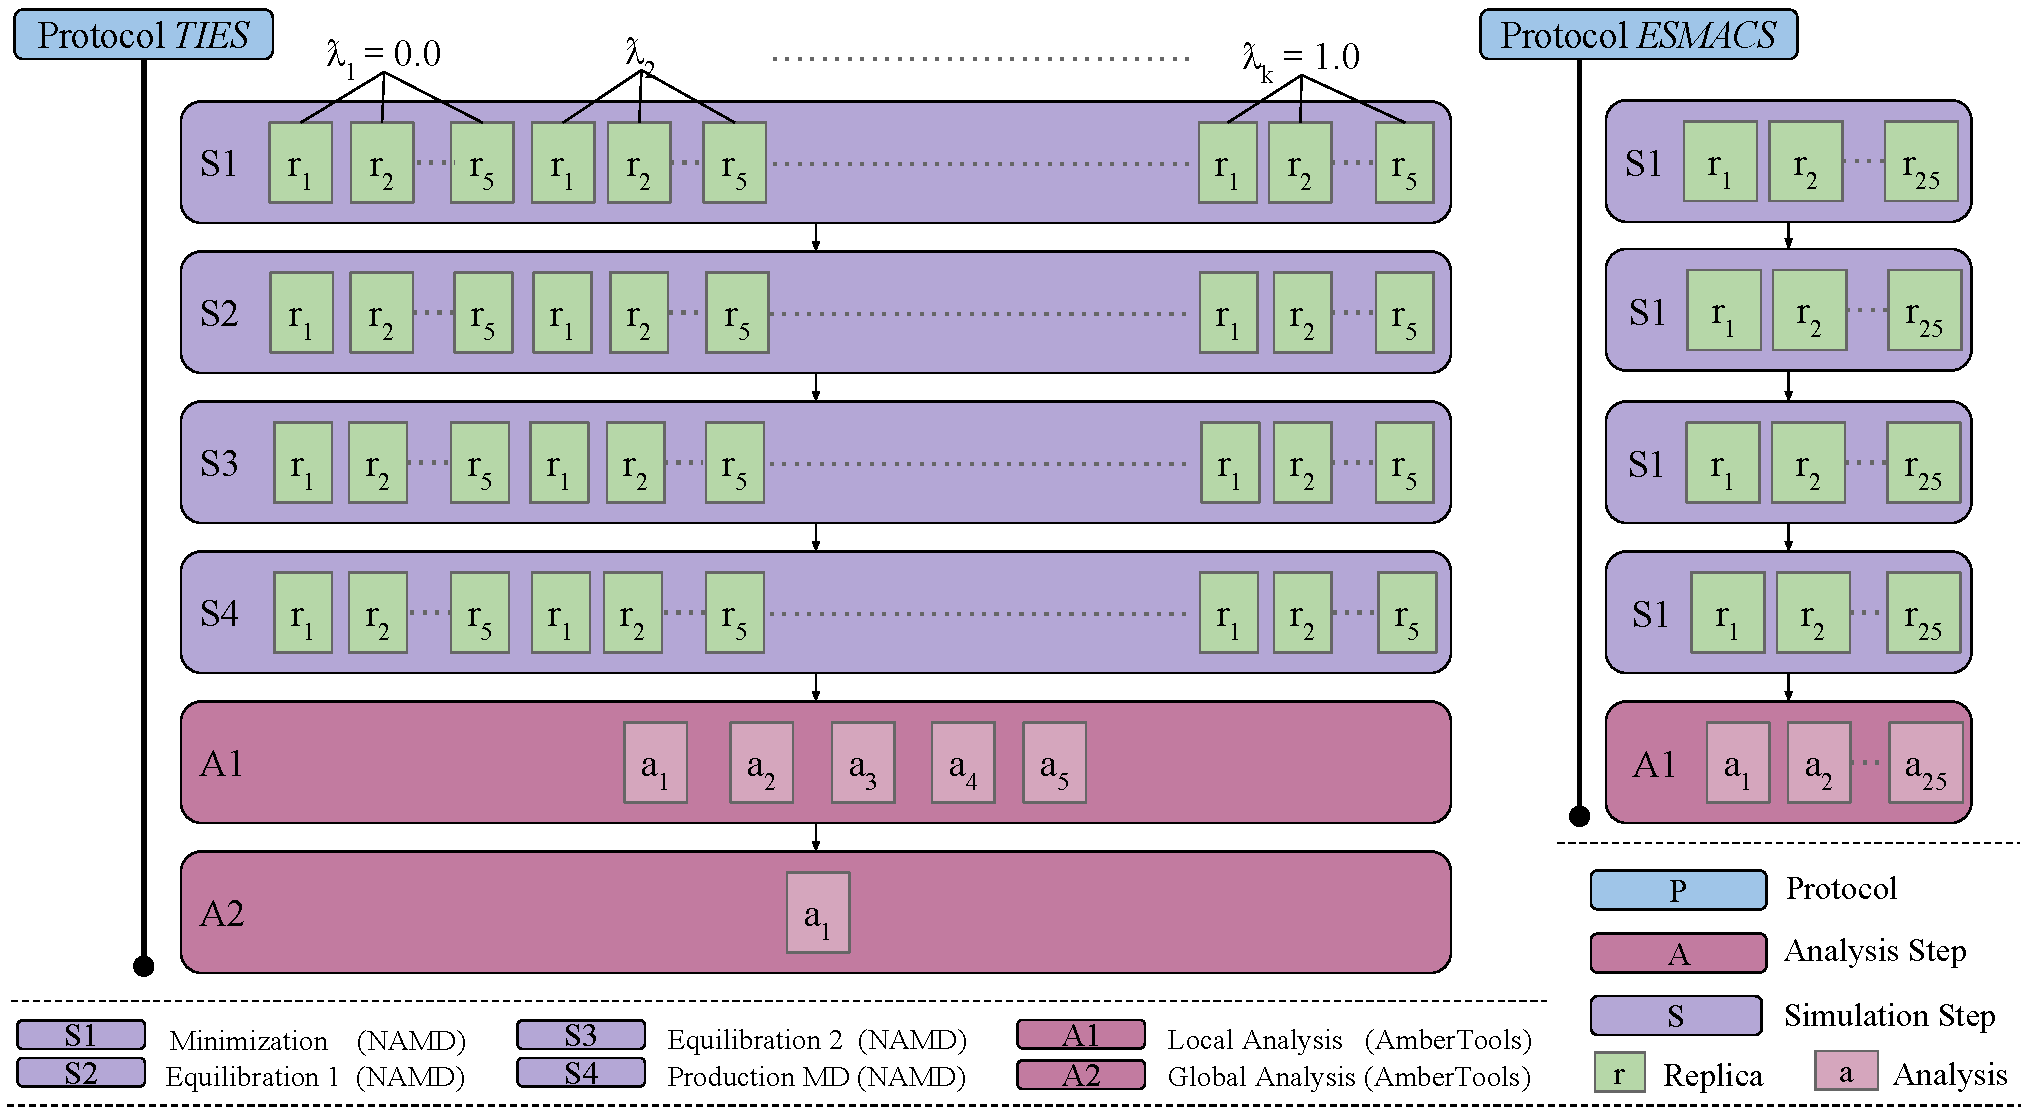
\includegraphics[width=\columnwidth]{figures/ties_esmacs_application_model.pdf}
  \caption{TIES and ESMACS protocols consist of simulations steps followed
  by analysis step(s). All replicas simulate for 6 nanosecond durations. 
  All replicas within a simulation step are assigned simulation timesteps 
  based on the \jdnote{UCL please provide the end of sentence}}
  % $S1=1000$; $S2=30,000$; $S3=800,000$; $S4=2,000,000$.}
\label{fig:ties_esmacs_application}
\end{figure}

%Adaptive quadrature is a numerical integration algorithm that is designed to
%minimize the number of function evaluations while still achieving a given error
%tolerance when estimating the integral. 
%We use this algorithm to minimize the
%number of full simulations that are required to be run, while still keeping the
%high accuracy of the protocol.

\subsection{The Value of Adaptivity}

Both ESMACS and TIES have been successfully used to predict binding affinities
quickly and accurately. Nonetheless, they are very expensive computationally,
and optimizing the execution time while still improving the accuracy is
desirable. Given the very large number of drug candidates, it is imperative to
gain maximum insight into potential candidate compounds using time and
resources efficiently. This provides one clear motivation for the use of
adaptive methods which minimize the compute time used whilst producing binding
free energy estimates meeting pre-defined quality criteria (such as
convergence or statistical uncertainty below a given threshold).
  
% Drug discovery programmes usually have limited resources, and require a
% resource budget carefully looking to gain maximum insight into potential
% candidate compounds. 

A second driver for adaptivity is that such algorithmic methods  will
typically involve compounds with a wide range of chemical properties which can
impact not only the time to convergence, but the type of sampling required to
gain accurate results. In general, there is no way to know before running
calculations exactly which setup of calculation is required for a particular
system. For example in TIES, the number (or the exact location) of the
$\lambda$ windows that will most impact the calculation are not known
\textit{a priori}, and change between physical systems (drugs). As multiple
simulations must be run for each window, sampling with a very high frequency
is expensive and impractical. Furthermore, adaptive placement of $\lambda$
windows is likely to better capture the shape of the 
$\partial U/\partial\lambda$ curve, leading to more accurate and precise 
results for a given computational cost.

On occasion, alchemical methods may be very slow to converge; in such
circumstances use of another method, such as ESMACS, may be the best option.
This means that the most effective way to gain accurate and precise free
energy results on industrially or clinically relevant timescales is to be able
to adapt both sampling (intra-protocol) and even the type of calculation 
(inter-protocol) used at run time. With potentially thousands of simulations, 
often employing multiple analysis methodologies, this provides the most 
effective way to utilize these techniques and resources at scale.

%-----------------------------------------------------------------------------%
% move this section to fe_protocols.tex

Intra-protocol adaptivity relies on the intermediate results \textit{within}
a protocol instance to define the next set of requirements. In this paper, we
use an intra-protocol adaptive implementation of TIES because, as indicated
in section~\ref{sec:science-drivers}, the optimal positions of the $\lambda$
windows are not known \textit{a priori}. Therefore, the number of simulations
and their descriptions, which are dictated by the $\lambda$ windows
parameter, cannot be specified before execution \mtnote{`cannot be specified'
or `cannot be effectively specified'? If the former, then would that imply
that a nonadaptive implementation is not possible?}.

Figure~\ref{fig:adaptive_ties} shows our implementation of TIES as a workflow
with an iterative pipeline of two stages: a simulation step followed by an
analysis step which determines optimal placement \mtnote{is placement the
correct term here? In the previous paragraph we wrote about number of
simulations and their description, not about their placement} of further
simulations. We initialize the workflow with $y$ evenly-spaced $\lambda$
windows, which generates $y \times n$ initial replicas. After the first
simulation step, the analysis step operates on the simulation results to
determine the next placement of $\lambda$ windows and to generate a second
simulation step with new configurations. 

Each simulation step consists of multiple tasks that simulates 1 nanosecond
of \ldots \mtnote{please add here what we are simulating}. The analysis
consists of a single task that computes adaptive quadrature calculations (as
defined in section~\ref{sec:science-drivers}) to determine whether to spawn
additional $\lambda$ windows \textit{in between} existing windows. This
enables continuous execution of existing simulations and beginning of new
simulations \mtnote{I do not understand this sentence. Can we eliminate it?}.
The workflow is executed iteratively until the total simulation duration
defined by the user is reached, determining termination.

\begin{figure}
  \centering
  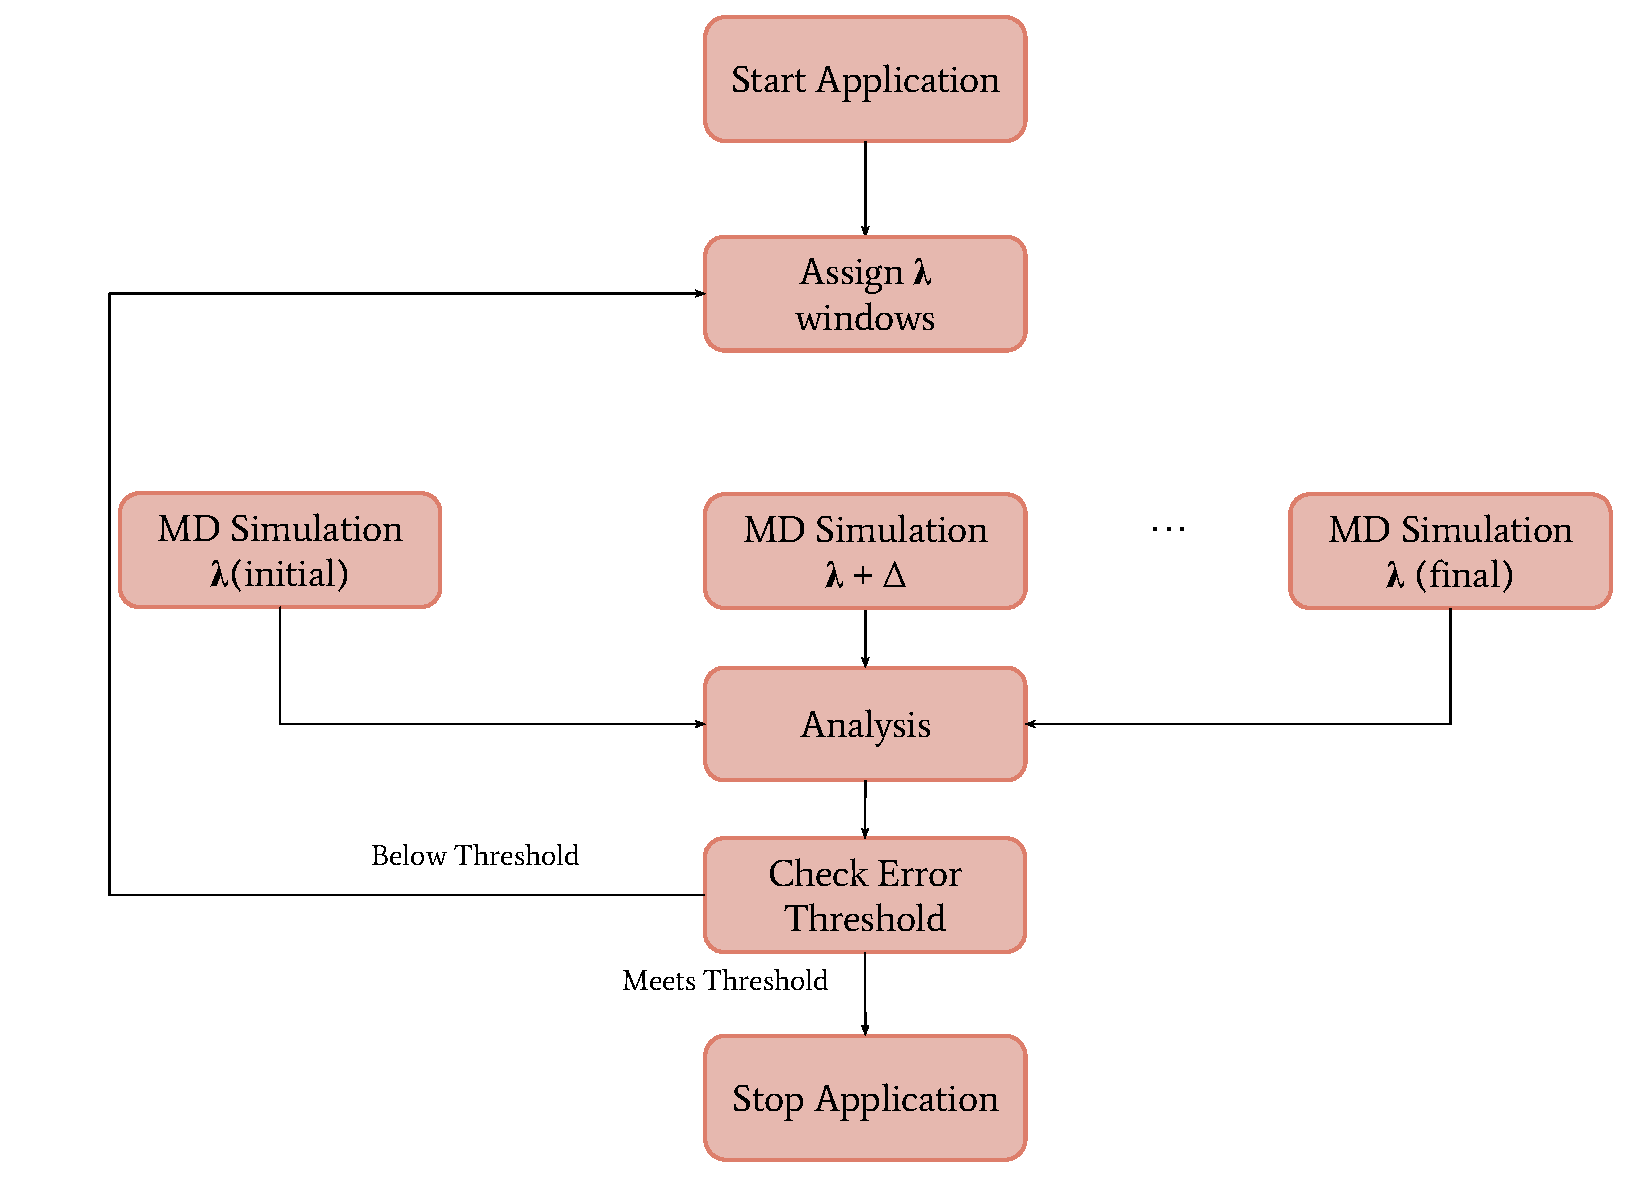
\includegraphics[width=\columnwidth]{figures/adaptive_TIES_workflow_diagram.pdf}
  \caption{Adaptive workflow of TIES with multiple concurrent and independent
  simulations. The analysis (adaptive quadratures) operates on a snapshot of
  the current simulations for each $\lambda$ window, and decides whether the
  critical threshold is reached, else current simulations continue executing
  and new simulations are spawned based on additional $\lambda$ values.}
\label{fig:adaptive_ties}
\end{figure}


\subsection{Target protein: BRD4}

Bromodomain-containing proteins, and in particular the four members of the BET
(bromodomain and extra terminal domain) family, are currently a major focus of
research in the pharmaceutical industry. Small molecule inhibitors of these
proteins have shown promising preclinical efficacy in pathologies ranging from
cancer to inflammation. Indeed, several compounds are progressing through
early stage clinical trials and are showing exciting early
results~\cite{Theodoulou2016}. One of the most extensively studied targets in
this family is the first bromodomain of bromodomain-containing protein 4
(BRD4-BD1) for which extensive crystallographic and ligand binding data are
available~\cite{Bamborough2012}.

We have previously investigated a congeneric series of ligands binding to
BRD4-BD1 (we shall from now on refer to this are simply BRD4) using both
ESMACS and TIES. This was performed in the context of a blind test of the
protocols in collaboration with GlaxoSmithKline~\cite{Wan2017brd4}. The goal
was to benchmark the ESMACS and TIES protocols in a realistic drug discovery
scenario. In the original study, we investigated chemical structures of 16
ligands based on a single tetrahydroquinoline (THQ) scaffold.
% ~\cite{Gosmini2014}. 
Here we focus on the first seven of these ligands to test
and refine the protocols used and the way in which they were executed. The
results of our previous work provide a benchmark of both accuracy and
statistical uncertainty to which we can compare our new results.

Initial coordinates for the protein-ligand system where taken from the X-ray
crystal structure PDB ID: 4BJX.
% ~\cite{Wyce2013}. 
This structure contains a
ligand based on the THQ template and other ligands were alligned with this
common scaffold. Preparation and setup of the simulations were implemented
using our automated tool, BAC~\cite{Sadiq2008}. This process including
parametrization of the compounds, solvation of the complexes, electrostatic
neutralization of the systems by adding counterions and generation of
configurations files for the simulations. The AMBER ff99SB-ILDN~\cite
{Lindorff-Larsen2010} force field was used for the protein, and TIP3P was used
for water molecules. Compound parameters were produced using the general AMBER
force field (GAFF)~\cite{Wang2004} with Gaussian 03
%~\cite{Frisch} 
to optimize compound geometries and to determine electrostatic potentials at
the Hartree–Fock level with 6-31G** basis functions. The restrained
electrostatic potential (RESP) module in the AMBER package~\cite{Case2005} was
used to calculate the partial atomic charges for the compounds. All systems
were solvated in orthorhombic water boxes with a minimum extension from the
protein of 14 \AA\ (the resulting systems contain approximately 40 thousand
atoms).


\section{HTBAC: Design and Implementation}
% ---------------------------------------------------------------------------
\subsection{Computational Challenges}


\jhanote{we need to elevate the challenge above (i) ensembles, (ii) and separate adaptive from non-adaptive challenges}


Most advances in high-performance computing have focused on the scale,
performance and optimization of single long simulations. However, due to the
end of Dennard scaling and methodological advances, many applications are now
formulated using multiple, shorter ensemble-based simulations. Yet, there are
limited software solutions that can execute scalable heterogeneous
computational tasks. Furthermore, statistically meaningful results derived
from simulations are of critical interest, as they can leverage additional
sampling of simulations which could lead to an improvement in precision 
of free energy calculations. Such decisions typically, cannot be made {\it a
priori} and require postmortem user intervention in order to analyze and spawn
additional simulations.

% To encode an algorithm into a set of tasks requires a workflow system that
% exposes an interface to describe tasks, dependencies, and an execution
% pattern. Once the algorithm is encoded into a set of tasks, the workflow
% system is required to translate tasks into executables, coordinate task
% dependencies, and acquire and manage resources.

%\jhanote{I'm changing the order of paragraphs: promoting adaptivity, as we
%seem to be building the case for decision making.}

% We define \textbf{adaptivity} as the ability to revisit a prior execution
% decision based on a runtime evaluation. Adapting workflows at runtime requires
% incorporating additional parallelism, redistributing of resources across
% tasks, and analyzing the performance and functionality of added adaptivity to
% evaluate its benefits and further design.

Many workflow management can be used to automate ensemble-based workflows but
suffer of several limitations. Among these, two of the most relevant are long
time to adoption and lack of dynamic capabilities.
% monolithic designs provide end-to-end capabilities to execute workflows on
% heterogeneous and distributed cyberinfrastructure. Other workflow systems
% entail
Workflow system with featureful but complex interface models impose
substantial overhead when integrating application workflows in the runtime
system, preventing users from quick and flexible applications prototyping.
Moreover, any intervention during runtime such as spawning additional 
simulations could require a redistribution of resources.  
% Furthermore, performance and resource utilization are necessary to ensure
% scalability of tasks, with minimal overhead in scheduling.
Current workflow management systems do not provide adequate
support for dynamic resource utilization, limiting the possibility to modify 
workflow models at runtime. 

% ---------------------------------------------------------------------------
\subsection{HTBAC}

In response to these challenges and requirements, and the absence of
middleware providing scalability and generality to applications for ensemble-
based protocols executed on HPC, we discuss the design and implementation of
HTBAC, which builds upon the RADICAL-Cybertools (RCT), a set of software
building blocks that eschew monolithic workloads. RCT is engineered to scale
across diverse computing platforms with the rapid ability to design a
multitude of workflows. HTBAC promotes biosimulation protocols to high-level
programming abstractions to enable the user to specify and efficiently grow
protocols, thereby enabling concurrent screening of drug candidates with the
added functionality to guide simulations in real-time.


Efficient execution of binding affinity calculation protocols on different
cyberinfrastructure poses several technical challenges, none of which are of
interest to domain scientists. \jhanote{too informal for my taste.} This
suggests three requirements for HTBAC\@: (1) enabling the execution of
multiple protocols on heterogeneous cyberinfrastructure; (2) abstract the
complexity of building protocols, execution and resource management from the
user; and (3) providing adaptive features to enables changes to the workflow,
i.e. the task-graph during runtime, based on decisions generated by previous
tasks.

%\jhanote{NEED DIAGRAMS ASAP}

% ---------------------------------------------------------------------------
\subsection{Implementation}

In section \ref{sec:science-drivers}, we described two examples of ensemble-based protocols (ESMACS/TIES)
where each protocol contains multiple simulation steps followed by multiple 
aggregate statistical analysis steps. Steps vary in data input dependencies, 
computational resource requirements and MD execution engines. We define 
each step as a computational \textbf{task} and the aggregation of these 
steps alongside their dependencies as a \textbf{workflow}. Subsets of 
these tasks are defined as \textbf{workloads}, i.e., tasks whose dependencies 
have been satisfied at a particular point in time and may be executed 
concurrently. Each protocols' ensemble requires an identical workflow 
with input parameter modifications.

HTBAC is a workflow system implemented in Python, and uses RCT as the runtime
system and to build ensemble-based workflows. Ensemble Toolkit (EnTK), the
topmost layer of RCT simplifies the process of creating ensemble-based
applications with complex coordination and communication requirements. The
EnTK API exposes the PST model which consists of three components:
\textbf{Pipeline}, \textbf{Stage}, and \textbf{Task}, in order to encode the
BAC protocols into workflows. Once the workflow is described, it is submitted
to the \b{Application Manager} which sets up multiple processes, threads and a
RabbitMQ message queue for communication. EnTK identifies tasks which have
dependencies satisfied and can be executed concurrently. EnTK's
\textbf{Execution Manager} uses the underlying runtime system, RADICAL-Pilot
to execute the tasks on specific target resources.


\begin{figure}
  \centering
   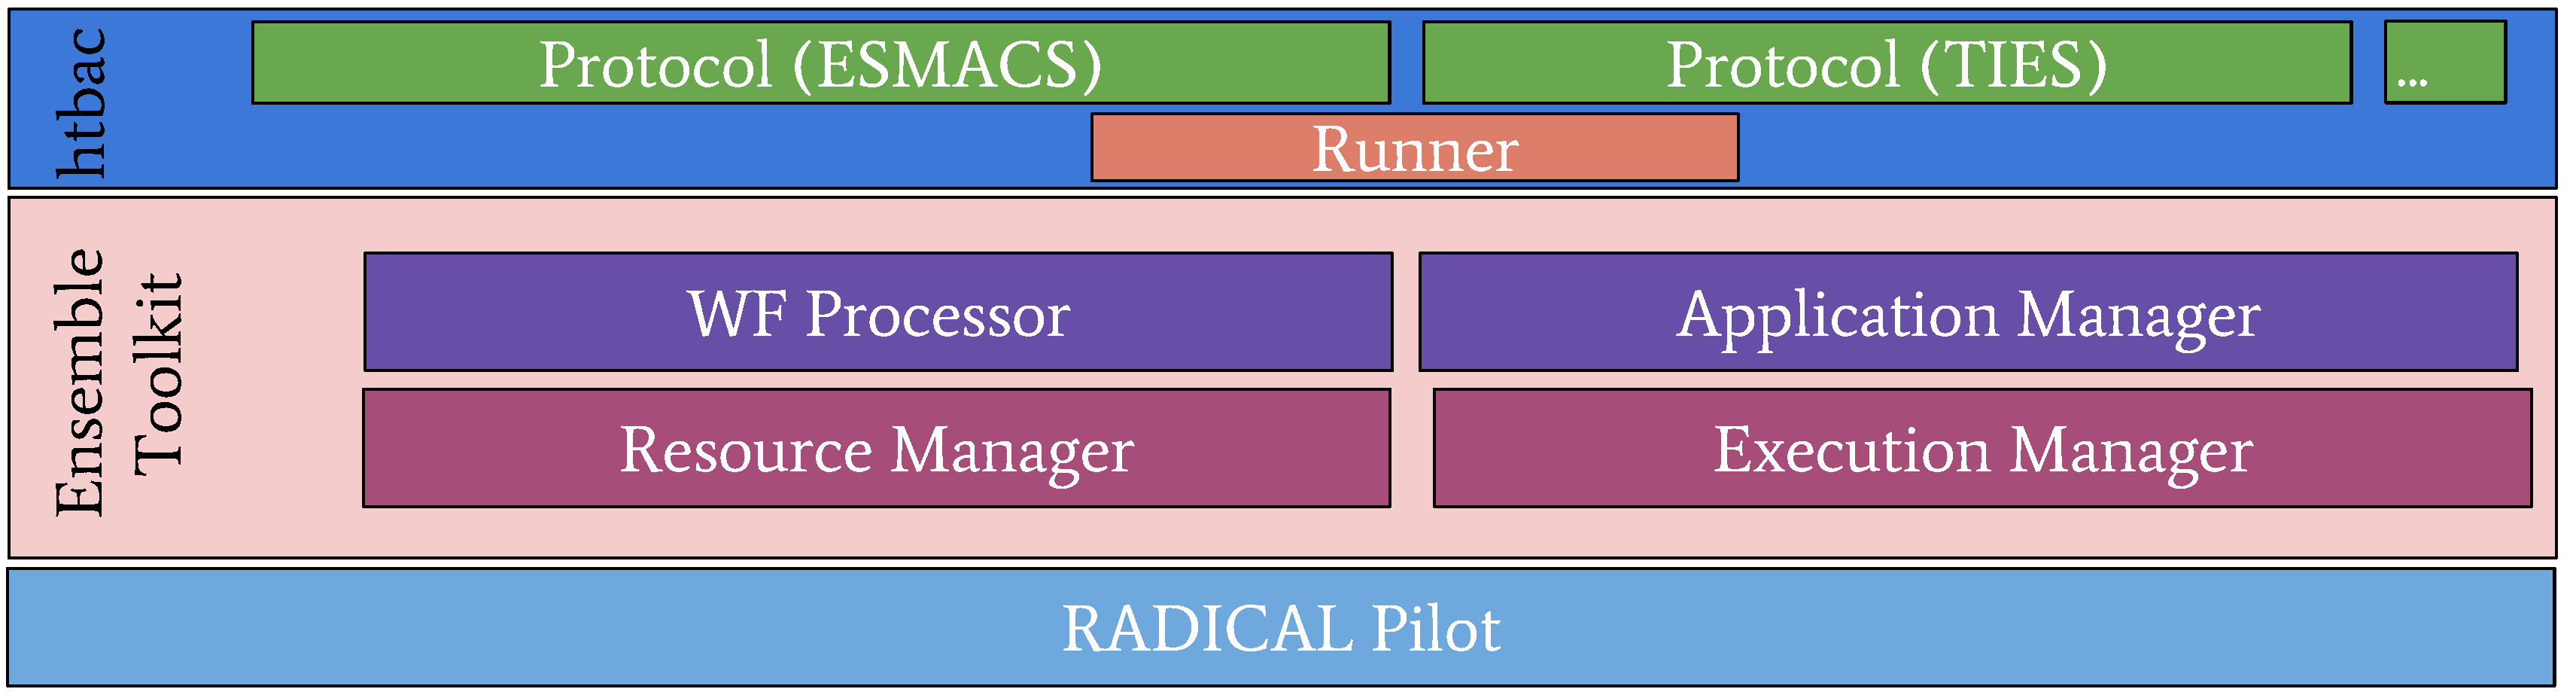
\includegraphics[width=\columnwidth]{figures/isc_htbac_integration_with_entk_RP.pdf}
  \caption{Mapping of flow between HTBAC, EnTK, and RP. The HTBAC API exposes the Protocol
  and Runner components. EnTK serves as the workflow execution system and
  by managing the workflow and workload. RADICAl-Pilot serves as the runtime system}
\label{fig:integration}
\end{figure}

	In our earlier work~\cite{dakka2017} we demonstrated how we applied the PST model to
implement the ESMACS protocol into an EnTK application. Here we expand upon this
work to further abstract the protocol implementation details and resource
information from the user. Domain scientists can leverage the generalization
of HTBAC and only need to define the ensemble parameters.

	HTBAC exposes two components \textbf{Runner Handle} and \textbf{Protocol}.
The \textbf{Runner} component is a container that implements the ESMACS 
and TIES into the EnTK PST model abstraction. The \textbf{Protocol} 
abstraction enables the user to select a protocol \textit{instance}, physical
system, number of replicas, core allocation per replica, and lambda 
windows (for alchemical pertubations). Currently the HTBAC abstraction provides
the ESMACS and TIES protocols. The user can scale protocol instances to study as
many physical systems as desired. The specification of protocols and 
their parameters are passed by the user to the \textbf{Runner Handle} which 
translates the request to EnTK. 

	In Section \ref{sec:related-work} we highlighted how an ensemble simulation 
approach can both aid sampling and provide improve uncertainty quantification 
for free energy calculations. Despite these crucial advantages, 
it remains non-trivial for field 
researchers to write biosimulation applications or protocols supporting 
multiple replica or multiple protocols in a given run. With HTBAC, this 
burden is minimized by specifying the number of replicas to the 
\textbf{Protocol} object, which determines the number of concurrent simulations. 
Moreover, the added ability to generate multiple protocols in a single interface 
enables the user to study a range of physical systems in a single run. 

%\jhanote{Is this specific to the TIES protocol or to the protocol class. Needs
%clarification.} 
%The same approach has been expanded to facilitate the creation of 
%sub-ensembles where the simulation configuration is altered programatically.
%An example of this is the implementation ofthe TIES protocol,
%where the user controls the $\lambda$ parameter values used in simulatios to 
%control which hybrid system states are sampled.

%A parameter, $\lambda \in [0, 1]$ is set for values between extremes and a
%simulation has to be run for every $\lambda$ value. The values form a function
%of energy and are integrated to obtain the desired results, the
%\emph{relative} binding free energy.


%\subsubsection{System}

%Systems This allows for multiple systems to be tested in the same
%\emph{single} run. A common scenario is the calculations of the binding
%affinity of a set of ligands with the same protein. System itself is just a
%collection of file paths pointing to descriptions of the system, like the
%system structure, topology etc. This class also provides the core/node
%requirments per single run, and reads some of the system descriptions from
%files to fill in the configuration settings.



%The Pipeline-Stage-Task (PST) framework developed by the Radical team
%(cite), and the Ensemble Toolkit (EnTK) built on top of it, offers a
%flexible way to express the molecular dynamics simulation workflows present
%in academia (cite) in terms of the radical pilot execution environment. Here
%we present a proposed mapping between the two (the PST and the MD layers)
%that is both simulation engine and protocol agnostic and allows for the
%compact expression of ensembles frequently used in binding affinity
%calculations.

%\subsection{Overview}

%The framework, called High Throughput Binding Affinity Calculator (HT-BAC),
%a python library, is made up of the following components: Workflow, Step,
%Ensembles and Simulation. These four object are all that is neccessary to
%describe the complex binding affinity caluculations in a generic way.

%\subsection{Workflow}

%The highest level abstraction is the Workflow. It is a container for the
%sequential units that are the simulation steps themselfs, and also contains
%meta-information about the job, like the resource description that the job
%will be running on, the total number of cores (nodes) required to fullfil
%the needs of the simulations and profiling mechanims to measure execution
%time.


% ---------------------------------------------------------------------------
%\jhanote{I don't these "description" should be subsections. Consider 
%"\paragraph{}"}

%\subsection{Step}

%\jhanote{what is a step? It is unclear to the reader. Is "step"  construct
%within HTBAC or is this just a description of the pipeline?}

%The workflow containts an ordered list of \emph{steps}. Steps give
%\jhanote{order?} orderd to the basic building blocks of binding affinity
%calculations. Usually they are (i) minimization (some form of local
%optimization of atom coordinates), (ii) heating, (iii) equilibration and (iv)
%production run.

%Additionally there is one or more steps of analysis at the end. The key
%point, is that these steps \emph{have} to be run consecutively, as they are
%dependent on the previous one. This is ensured by the \texttt{Stage} objects
%of EnTK\@. Each step has list of \texttt{Ensemble}s and a \texttt{Simulation}
%object.

% ---------------------------------------------------------------------------
%\subsection{Ensembles} 

%\jhanote{I'm not sure what we are trying to do here. We've just described
%the abstract/constructs in HTBAC to be protocols. Why are we regressing to
%presenting Ensembles as a construct in HTBAC, when they are a construct of
%EnTK?}

%Ensembles in HTBAC are a powerful construct that allows for extreme
%generalizations. At their core they are a nondestructively multi (forward)
%traversable \emph{iteratable}s. The underlying iterator yields a function that
%modifies a \texttt{Simulation} object to reflect the current state of the
%ensemble. This is similar to the iteratee construct, the only difference being
%that the function is applied to the \emph{same} data consecutively (as opossed
%to chunks of a stream of data).

%The Simulations are then generated for every Step based on what ensembles are
%attached to it. This is done by taking the \texttt{product} of all the
%ensembles, meaning that we go over every possible combination of ensemble
%states, and create a simulation from it. This is equivalent to an $n$ level
%deep for-loop, where $n$ is not known beforehand.

% ---------------------------------------------------------------------------
%\subsection{Simulation}

%Simulation is the lowest level building block. \jhanote{The use of building
%block for simulation will confuse the reader as it is overloading the term.
%Find alternative description.} It maps to the \texttt{Task} object in the PST
%model, and deals with executing the simulation engine, collecting input for
%it, and modifing the configuration of the simulation to reflect the ensembles
%that it is in.

%The main driver of a simulation is the configuration file. This file
%containts the specific settings of the Molecular Dynamics simulation,
%including the thermostat, barostat, constraints, long range force calculation
%methods and more. Some of the settings are general and apply to every
%simulation of a given step, but some are specific to the Ensemble that the
%simulation is in. After the ensemble modifies properties of the Simulation,
%these get propagated and written to the configuration file to be read by the
%executable.

% ---------------------------------------------------------------------------
%\subsection{Sandboxing}

%Sandboxing mechanims are built into the Radical stack for every layer. Each
%separate run has it's own sanbox, and inside each run, all the Tasks have
%their own sandbox too. This means that there is no unintented interference
%between Tasks, and data can be confidently analyised inside each sandbox.
%This mechanism also simplyfies the input data referencing, as the input in
%\emph{guaranteed} to be in the sandbox, and can be referenced relative to it.
%We recommend this sandboxing system for all simulations.

% ---------------------------------------------------------------------------
%\subsubsection{Data flow}

%while sandboxing offers a powerful way to separate the simulations, by the
%inherent nature of workflows, output data from one simulation is required as
%input for the next one. Simulation objects can find their previous
%couterparts by way of the ensemble that they are in. Then data is transfered
%via \textbf{copy-on-demand}, i.e. data is copied \emph{only} if it is known
%to be edited during execution, otherwise only a symbolic link is created to
%point to the original location of the file. This drasticly reduces the copy
%overhead, while still keeping the sandboxes separate.

% ---------------------------------------------------------------------------
\subsection{Adaptability}

%Once we tackle the barrier between the local workflow creation and the remote
%execution, new features become availble, and readily usable by scientists.
%Intraprotocol adaptability is one such new feature.

% ---------------------------------------------------------------------------
\subsubsection{Intraprotocol adaptability}

%while conceptually simple, tradiational execution patters used in academia
%makes this very hard. In HTBAC variables like replica size, specific lambda
%windows or simulatable system are settable on demand, the execution of which
%is automatically handeled by the library. To illustrate: a common scenario is
%the non adequate convergence of the statistical results after running a given
%number of replicas. In HTBAC the replica number can be changed, rerun and the
%results reevaluated. Additionally, logic can be written, to dynamically add
%more replicas until a given convergence tolerance has been reached.


\vspace{-0.2in}

\section{Experiments}
Design and Methods

Weak Scalability Design:

Both ESMACS and TIES protocols consist of pipelines that represent replicas. The ESMACS protocol requires 25 pipelines, while TIES requires 65 pipelines. In both protocols, each pipeline contains four stages. Each stage contains a single task. EnTK manages the queueing of the tasks in accordance with the order and concurrency mandated by stages and pipelines: For each pipeline, each stage is executed sequentially while pipelines are executed concurrently.

We previously demonstrated weak scaling of the ESMACS protocol in [ref SC] where we showed that a single ESMACS instance could run up to 128 concurrent pipelines. In here we expand upon this work to show weak scalability for growing the number of protocol instances while adhering to the required number of pipelines for each protocol. By design of each protocol, an increase in the number of instances simply means an increase in the number of pipelines. Therefore our previous ESMACS experiment referenced in [ref SC] already demonstrates the scalability of ESMACS as a growth in the number of pipelines.

The first weak scalability experiment demonstrates the behavior of HTBAC, EnTK and RP using the multiple instances of
the TIES protocol. By design of weak scaling, the ratio between the number of pipelines and cores are kept constant. At every scale we introduce twice as many protocol instances. The goal is to isolate and understand
the impact of increasing the number of instances, thereby the execution workload.

The next weak scalability experiment replicates the design of the first experiment using a combination of TIES and ESMACS instances. The comparison of experiment 1 and 2 shows the ability to execute procotols with different resource requirements using one pilot.

Strong scalability design: Next we repeat the same design of the weak scalability experiments but examine performance of strong scaling when fixing the number of pipelines and varying the resources. The comparison between weak and strong scalability demonstrates the overhead introduced by load balancing and scheduling tasks in multiple generations.

%Strong scaling argument: If you go big enough you start to encounter high rates of failures on the machines. Part of the reason to do both is to find the sweet spot between weak/strong scaling.

Experimental Setup

We perform weak (and strong) scalability experiments on NCSA Blue Waters--a 13.3. petaFLOPS Cray, with 32 Interlago cores/50 GB RAM per node, Cray Gemini, Lustre shared file system.

Overhead of HTBAC, EnTK and RP

EnTK consists of multiple active components interacting with each other in order to support the execution of ensemble based applications. This process includes various events such as validation of the workflow, validation of the resource description, submission of resource request, creation of tasks, translation of tasks to and from the runtime system amongst several others. In order to understand the contribution of the various events in Ensemble Toolkit, termed as EnTK overhead, to the total time to run, we construct the following experiments.

Time to run = T(overhead\textsubscript{entk}) + T(overhead\textsubscript{rp}) + T(execution)


%\section{Results}
%%------------------------------------------------------------------------------
<<<<<<< HEAD

\subsection{Performance Characterization}

...


\subsubsection{Weak Scaling Experiments}

%We previously demonstrated weak scaling of the ESMACS protocol in [ref SC] where we showed that a single ESMACS instance could run up to 128 concurrent pipelines.
%\jhanote{1 sentence about how pipelines in ESMACS were simpler than TIES? else the
%reader will say: you did 128 pipelines already... why should I be impressed by a
%small number of pipelines. Important to highlight that the scalability is over
%PROTOCOL INSTANCES and not pipeline instances.} \jdnote{added blurb in
%design \& implementation, removed it from here}

Here we show weak scalability for the TIES protocol by growing the number of
protocol instances while adhering to the required number of pipelines. By
design of each protocol, an increase in the number of instances simply means
an increase in the number of pipelines. Therefore our previous ESMACS
experiments~\cite{} \jhanote{fix please} demonstrates the scalability of
ESMACS as a growth in the number of pipelines.

The first weak scalability experiment demonstrates the behavior of HTBAC, EnTK
and RP using the multiple instances of the TIES protocol. By design of weak
scaling, the ratio between the number of pipelines and cores are kept
constant. As the number of cores (measure of resource) changes by a factor of
2, we introduce twice as many protocol instances. As designed, the weak
scaling property provides insight into the size of the workload that can be
investigated in a given amount of time.


% The goal is to isolate and understand the impact of
% increasing the number of instances, thereby the execution workload.



%The next weak scalability experiment replicates the design of the first experiment using a combination of TIES and ESMACS instances. The comparison of experiment 1 and 2 shows the ability to execute procotols with different resource requirements using one pilot.

\subsubsection {Strong Scaling Experiments}

Next we repeat the same design of the weak scalability
experiments but examine performance of strong scaling when fixing the number of
pipelines and varying the resources. The comparison between weak and strong
scalability demonstrates the overhead introduced by load balancing and
scheduling tasks in multiple generations.


\subsection{Validation experiments}
=======
\subsection{Weak/Strong Scaling Performance Results}

For the weak/strong scaling results, we first characterize the overheads of HTBAC and
the runtime system. HTBAC enables concurrent execution of multiple protocol instances.
With each new protocol instance generated for an
application, the HTBAC overhead grows to match the additional
requirement of generating and coordinating protocols. In order
to understand the contribution of the various events in HTBAC,
termed as HTBAC overhead, to the total time to run, we construct the following metrics:
\(Time-to-run = T(overhead\textsubscript{HTBAC} +
T(overhead\textsubscript{entk}) +
T(overhead\textsubscript{rp}) + T(execution)\). We define \(T(execution)\) as \(TTX = TTC - T_q\) where \(TTC\) is
time-to-completion and \(T_q\) is time spent queuing on the HPC machine.

The HTBAC overhead accounts for approximately 0.1\% of \(TTX\).
The remaining overheads, mainly EnTK and RP, depend on the number of tasks that need to be
translated in-memory from a Python object to a compute unit (CU) description. As such, it is
expected to grow proportionally to the number of tasks. EnTK submits CU descriptions to a
MongoDB used by RP, and the RP pilot pulls these descriptions from the same database.
This pull operation occurs over a wide area networks, which introduces varying amounts of latency.
In addition, each Stage constructed by EnTK maintains sequential barriers. As such, RP remains
dormant until completion of the current Stage before staging the next State. The impact of the 
barrier increases with number of CUs as seen in the 16 protocol instances datapoint 
in \ref{fig:weak_scaling}. 
Together, these two factors introduce delays in the scheduling of the CUs and results in 
higher overheads. 

 \(TTX\) measures the execution duration across all task, including file staging, MD kernel execution, 
 and post-executables. As a result, we expect an increase in \(TTX\). As such, each additional 
 protocol instance contributes to roughly 55 additional seconds in \(TTX\). 

 (Add in additional points on strong scaling if they come in)


\subsection{Validation Experiment Results}
>>>>>>> e0352a35ec687a5fcb233c81c82ab6029aa7fbe4

HTBAC fully automates the process of calculating the binding affinity of
protein-ligand complexes from reading the input all the way to analyising the
final results. In order to validate the correctness of the results, we have
devised a set of experiments. These experiments are vital to gain confidence
in the algorithm and to prove that it is indeed calculating the correct values.

The validation experiments were based on the original study of Wan et. al.
\cite{Wan2017brd4}. We selected a subset of the protein ligand systems that
were the subject of that study: they are the ligand transformations 3 to 1, 4,
and 7. We then performed a full simulation on all 3 systems and calculated the
binding affinity (see Table~\ref{tab:exp2}) using HTBAC.

The results show that all three $\Delta \Delta G$ values are within error bars
of the original study, reinforcing the fact that HTBAC has indeed correctly
implemented the complex workflow of TIES.

\begin{table}
  \centering
  \begin{tabular}{l@{\hskip 1in}r@{\hskip 0.2in}r@{\hskip 0.2in}r}
    \toprule
    System & HTBAC & Wan et. al & Experiment \\
    \midrule
    BRD4 \textbf{3 to 1} & \num{0.39 +- 0.10} &   \num{0.41 +- 0.04} &  \num{0.3 +- 0.09} \\
    BRD4 \textbf{3 to 4} & \num{0.02 +- 0.12} &   \num{0.01 +- 0.06} &  \num{0.0 +- 0.13} \\
    BRD4 \textbf{3 to 7} & \num{-0.88 +- 0.17} &  \num{-0.90 +- 0.08} & \num{-1.3 +- 0.11} \\
    \bottomrule
  \end{tabular}

  \caption{Comparison of the calculated binding free energies using HTBAC, from
  the original study by Wan et. al and experimental data. The two theoretical
  studies used the same protcol in principle. This experiment proved that HTBAC
  has indeed implemented TIES correctly, as the calculated values are either
  the same or within error bar of the original study. All values are in
  \textbf{kcal mol\textsuperscript{-1}}.}
  \label{tab:exp2}


\end{table}

%------------------------------------------------------------------------------

\section{Adaptive Quadrature Experiments Results}



\begin{figure}
\begin{tikzpicture}
\begin{axis}[
  xlabel=$\lambda$,
  ylabel=$\frac{dU}{d\lambda}$,
  xmin=0,
  xmax=1,
  legend pos=outer north east,
  grid=both,
  ]
  \addplot+[name path=alch_1, mark size=1pt, mark=*, color=blue] table [x=lambda, y=p1v]{figures/alch_1.csv};
  \addlegendentry{Iteration 0: inital lambda spacing};

  \addplot+[name path=alch_2, mark size=1pt, mark=*, color=red] table [x=lambda, y=p1v]{figures/alch_2.csv};
  \addlegendentry{Iteration 1: Increasing number of lambda values};

  \addplot+[name path=alch_3, mark size=1pt, mark=*, color=brown] table [x=lambda, y=p1v]{figures/alch_3.csv};
  \addlegendentry{Iteration 2: Optimial number of lambda values found};

  \addplot+[name path=alch_4, mark size=1pt, mark=*, color=black] table [x=lambda, y=p1v]{figures/alch_4.csv};
  \addlegendentry{Iteration 3: Refining function values at optimial mesh};

  \addplot[name path=line, draw=none] {0};

  \addplot fill between[
    of = alch_1 and line,
    split,
    every even segment/.style = {pattern color=blue!50, pattern=vertical lines},
    every odd segment/.style = {pattern color=blue!50, pattern=vertical lines},
    soft clip={domain=0:1},
  ];

  \addplot fill between[
    of = alch_2 and line,
    split,
    every even segment/.style = {pattern color=red!50, pattern=horizontal lines},
    every odd segment/.style = {pattern color=red!50, pattern=horizontal lines},
    soft clip={domain=0:1},
  ];

  \addplot fill between[
    of = alch_3 and line,
    split,
    every even segment/.style = {pattern color=brown!50, pattern=north east lines},
    every odd segment/.style = {pattern color=brown!50, pattern=north east lines},
    soft clip={domain=0:1},
  ];

\end{axis}
\end{tikzpicture}
\caption{The adaptive algorithm reevaluates the efficiency of the lambda window mesh after every \SI{1}{\nano\second} and makes a decision whether to place more lambda windows inside certain ranges. The decision of placing more lambda windows in a range $[\lambda_{i}; \lambda_{j}]$ is based on the following criterion: $|f(\lambda_{i})-f(\lambda_{j})| \leq h$ where $h$ is some threshold set by the user. Once the optimal mesh is reached, and no more lambda windows are needed, the algorithm runs the simulation for a further \SI{2}{\nano\second} to converge the results.}
\label{fig:adapt}
\end{figure}


\vspace{-0.2in}

\section{Discussion and Conclusion}
Ensemble-based protocols provide are showing considerable predictive
potential in computational drug campaigns. As drug screening can cover
millions of compounds and hundreds of millions of core-hours, it is important
for binding affinity calculations to optimize the accuracy and precision of
results obtained from a given set of resources. However, the optimal protocol
for a given system is difficult to determine {\it a priori}, thus requiring
runtime adaptation to workflow executions. We introduce HTBAC to enable
scalable and adaptive binding affinity energy calculations on HPC.

Specifically, this paper makes the following contributions: (1) shows
adaptive approaches within a ensemble-based free energy protocol (TIES) to
improve binding affinity accuracy given a fixed amount of computing
resources; (2) characterizes HTBAC, the software systems we developed to
address the aforementioned requirements; and (3) shows the capability to
execute adaptive applications at scale, validating their scientific results.

We characterize the performance of HTBAC on NCSA Blue Waters. We show
near-ideal weak and strong scaling behavior for ESMACS and TIES, individually
and together, reaching scales of 21120 cores. Furthermore, we validate
binding free energies computed with HTBAC with both experimental and
previously published computational results.

We compare computational consumption and free energy accuracy in our adaptive
and non-adaptive TIES results. Using the adaptive quadrature algorithm, we
show improvements in $\Delta \Delta$G on average by 77\% over the 5 physical
systems tested. By reducing the $\lambda$ windows on average by 32\%, we
reduce execution time by the same amount. The adaptive termination
implementation of the TIES protocol saves compute resources and reduces time
to solution on average by 16\%. To the best of our knowledge, adaptive TIES
protocols have not been benchmarked against non-adaptive implementations
before.

% ---------------------------------------------------------------------------
\subsubsection*{Software and Data}

{\footnotesize All experimental data can be found at
\url{https://github.com/radical-experiments/htbac-escience-18}. HTBAC (MIT
license) can be found at: \url{https://github.com/radical-cybertools/htbac}}

% ---------------------------------------------------------------------------
\subsubsection*{Acknowledgements}

{\footnotesize JD acknowledges Dept. of Education Award P200A150217 for her
fellowship. PVC acknowledges the support of the EU H2020 CompBioMed (675451),
EUDAT2020 (654065) and ComPat (671564) projects. Access to Blue Waters was
made possible by NSF 1713749. The software capabilities were supported by
RADICAL-Cybertools (NSF 1440677). We thank Vivek Balasubramanian and Andre
Merzky for support with RADICAL-Cybertools.}


\vspace{-0.2in}

\subsubsection{Software and Data: }
{\footnotesize All experimental data and analysis is available: 
\url{https://github.com/radical-experiments/isc-htbac-experiments}. 
HTBAC (MIT license) can be found at:
\url{https://github.com/radical-cybertools/htbac}}

\vspace{-0.2in}

\subsubsection{Acknowledgements}
%\input{acknowledgements}

{\footnotesize JD acknowledges Dept. of Education Award P200A150217 for her fellowship. PVC
would like to acknowledge the support of the EU H2020 CompBioMed (675451),
EUDAT2020 (654065) and ComPat (671564) projects. We thank Andre Merzky and
other members of the RADICAL team for support. Access to Blue Waters was made
possible by NSF 1713749. The software capabilities were supported by
RADICAL-Cybertools (NSF 1440677).}

\newpage

% ---------------------------------------------------------------------------
% BIBLIOGRAPHY
% -------------------,--------------------------------------------------------
\bibliographystyle{IEEEtran}
\bibliography{rutgers,ucl}

\end{document}
